Zur Bestimmung von Richtungs- und Diffusanteil werden zunächst Schallschnelle und Energie berechnet. Die Schnallschnelle wird als Vektor $\textbf{V}_{m}[k] = [X_{m}[k], Y_{m}[k], Z_{m}[k]]$ aus den gerichteten Anteilen (der Druckgradienten-Mikrofone) des B-Format Signals bestimmt. Der Schalldruck ist schlicht der omnidirektionale Anteil $W_{m}[k]$. Die Indizes $m$ und $k$ werden hier zur Kennzeichnung des Zeitfensters als Funktion der Frequenzzahl $k$ verwendet.

Die Schallintensität $\textbf{I}_{m}[k]$ wird aus dem Schnellevektor und dem konjugiert komplexen Schalldruck in Gleichung \ref{eq:inten} abgeleitet, wobei hier rein der Realteil heranzogen wird, da sonst die Blindeinteile des Schnellevektors das Ergebnis verfälschen würden. Der Intensitätsvektor stellt bereits die Schalleinfallsrichtung für alle Frequenzbins einzeln dar, jedoch entgegengesetzt der Einfallsrichtung $\textbf{D}_{m}[k]$ :

\begin{equation}
    -\textbf{D}_{m}[k] = \textbf{I}_{m}[k] = \Re(W_{m}[k]^{*} \cdot \textbf{V}_{m}[k])
    \label{eq:inten}
\end{equation}

Die Schallenergie $E_{m}[k]$ wird mit Hilfe von Gleichung \ref{eq:energy} ausgewertet:

\begin{equation}
    E_{m}[k] = \frac{|W_{m}[k]|^2+||\textbf{V}_{m}[k]||^2}{2}
    \label{eq:energy}
\end{equation}

Um Sprünge in der Lautsprecherzuordnung von gerichteten Signalen bei raschen Bewegungen zu vermeiden, wird der Intensitätsvektor zusätzlich durch eine zeitliche Mittelwertbildung geglättet. Diese Glättung kann im Skript mit einer frequenzabhängigen Zeitkonstante vorgegeben werde. Zusätzlich wird auch der Energievektor zeitlich geglättet. Anschließend wird der Intensitätsvektor verwendet, um die Einfallsrichtungen in sphärischen Koordinaten zu bestimmen.

Die Diffusität $\psi_{m}[k]$ kann schlussendlich aus dem Vergleich des Betrags des Intensitätsvektors mit der Energie ermittelt werden (Glg. \ref{eq:diff}). Der Erwartungswert entspricht hier den (zeitlich) gemittelten Vektoren.

\begin{equation}
    \psi_{m}[k] = \sqrt{1 - \frac{||\mathbb{E}(\textbf{I}_{m}[k])||}{\mathbb{E}(E_{m}[k])}}
    \label{eq:diff}
\end{equation}

\begin{figure}[!ht]
  \centering
  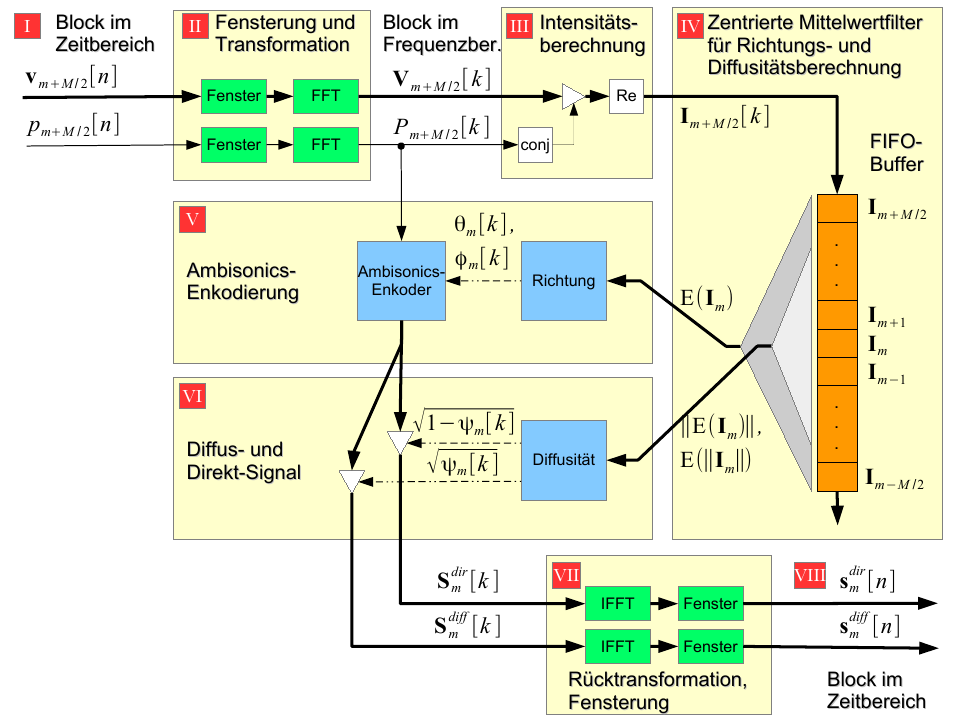
\includegraphics[width=0.7\textwidth]{implementierung/plots/flow.png}
  \label{fig:flow}
  \caption{Flussdiagram des DirAC Algorithmus in Octave\protect\footnotemark}
\end{figure}

\footnotetext{Quelle: \cite{seminar2016}}
